\chapter{Design Analysis}
An algorithm is the idea behind a program. An algorithm can be implemented in multiple ways leading to varying performance and efficiency of the program, for example, using different data structures, data storage options i.e. if the data should be stored in memory or on file system, implementation language, library functions used etc. A design is a result of such numerous decisions which are made during the development process.  Very rarely is it possible to find the perfect design which would lead to a program performing with the same efficiency for the entire input space. Hence, while making the decisions it is important to evaluate the advantages and disadvantages of the chosen approach. This chapter is therefore dedicated to analyze the design choices made during the implementation. 

\section{Application of distributed computing}

As discussed in section \ref{sysMod}, the task submitted by the user to the master node is divided into sub-tasks and distributed among the slaves nodes of the cluster. The slave nodes perform the allocated work and report the partial output which is merged at the master node. The flowchart \ref{lst:FC} summarizes the process. The \textit{MasterPrintingSoftware} follows the steps denoted in the left branch of the flow chart where as the \textit{SlavePrintingSoftware} follows the steps of denoted in the right branch of the flow chart. The \textit{MasterPrintingSoftware} and \textit{SlavePrintingSoftware} design decisions include:
\begin{enumerate}
\item Format of the sub-tasks allocated to the slaves nodes
\item Distribution of sub-tasks by the master
\item Format of the slave partial output 
\item Merging of the partial output 
\end{enumerate}

Each of the design possible from the combinations of the above decisions yields a different behavior of the component responsible for that particular task. The following section describes the two designs in detail implemented through the thesis.  

\section{Prototype I- Input/Output using NFS }

Prototype I is the base prototype wherein the nodes communicate amongst each other the input and the partial output using the shared networked file system. The synchronization amongst the nodes is done via message passing. 

\subsection{Master sub-task creation and distribution}
User submits the job to the master node using a configuration file in \textit{JSON} format. The JSON document contains a member called as \textit{PrintObjectFiles} whose member values indicate the geometry, texture, orientation etc of the object to be printed. The \textit{FileParserPJ} component of \textit{MasterPrintingSoftware} parses the input and converts it into an internal mesh representation called as the print object, with each having it's own unique identifier. The print objects are grouped together into a print job. Each print job is the organized in the print tray and then passed to the \textit{MasterDistributor} component which is in charge of sub-task creation and distribution. The sub-tasks distributed by the component can be already created print jobs or they can be in the same format as the received input i.e. configuration file. In this prototype, the \textit{MasterDistributor} creates a configuration file for each slave with the exactly same format as the configuration file parsed by the \textit{FileParserPJ} with a few changes i.e. the \textit{PrintObjectFiles} contains details of only the print models allocated to that particular slave and the \textit{OutputFolder} value is the folder location for the slave to write the partial output. In the figure \ref{fig:MasterConfigurationFile}, the configuration file received by the master node has the \textit{PrintObjectFiles} containing four inputs models which are distributed by the master as seen in the figure \ref{fig:Slave1ConfigurationFile} for the slave with rank 1 and figure \ref{fig:Slave2ConfigurationFile} for slave with rank 2. 

\begin{figure}[ht!]
\centering
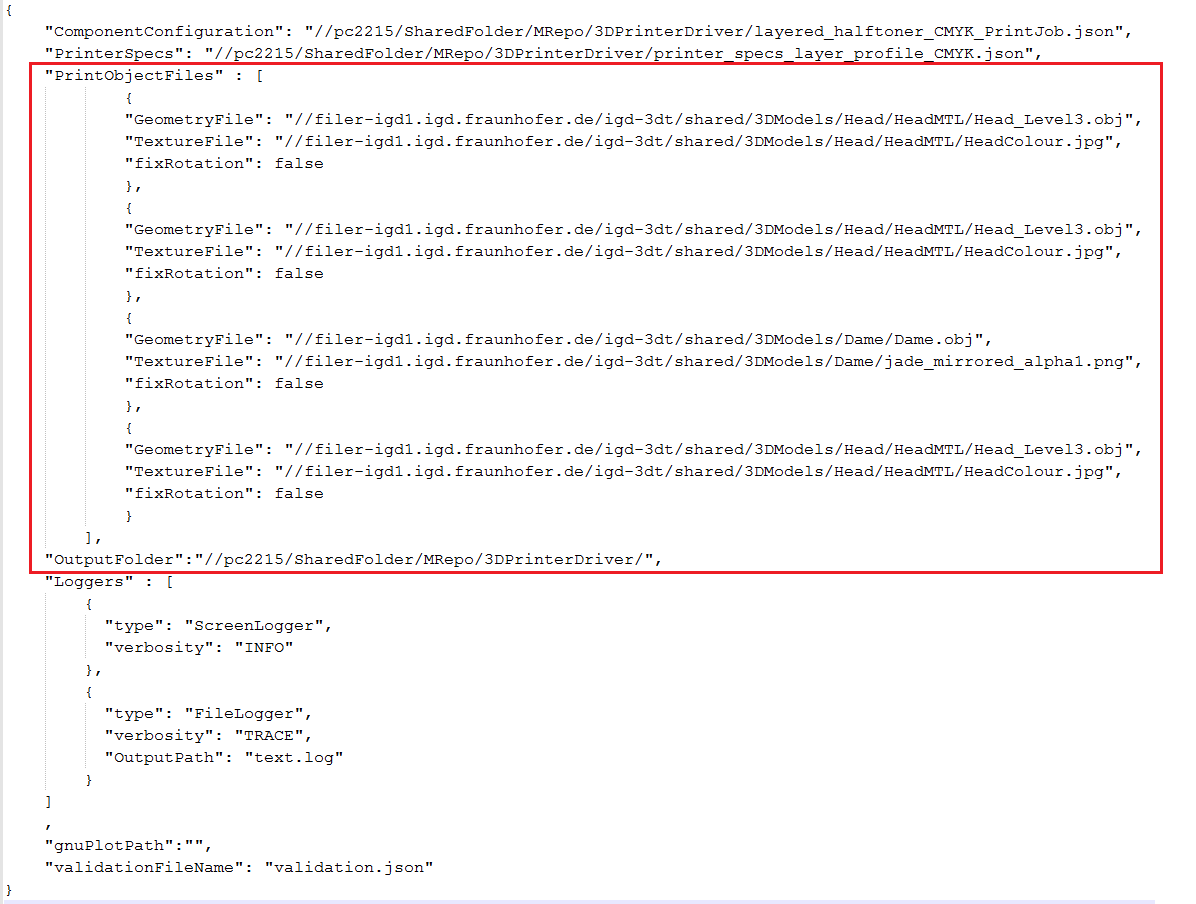
\includegraphics[scale=0.75]{MasterConfigurationFile.png}
\caption{Master Configuration file}
\label{fig:MasterConfigurationFile}
\end{figure}

\begin{figure}[ht!]
\centering
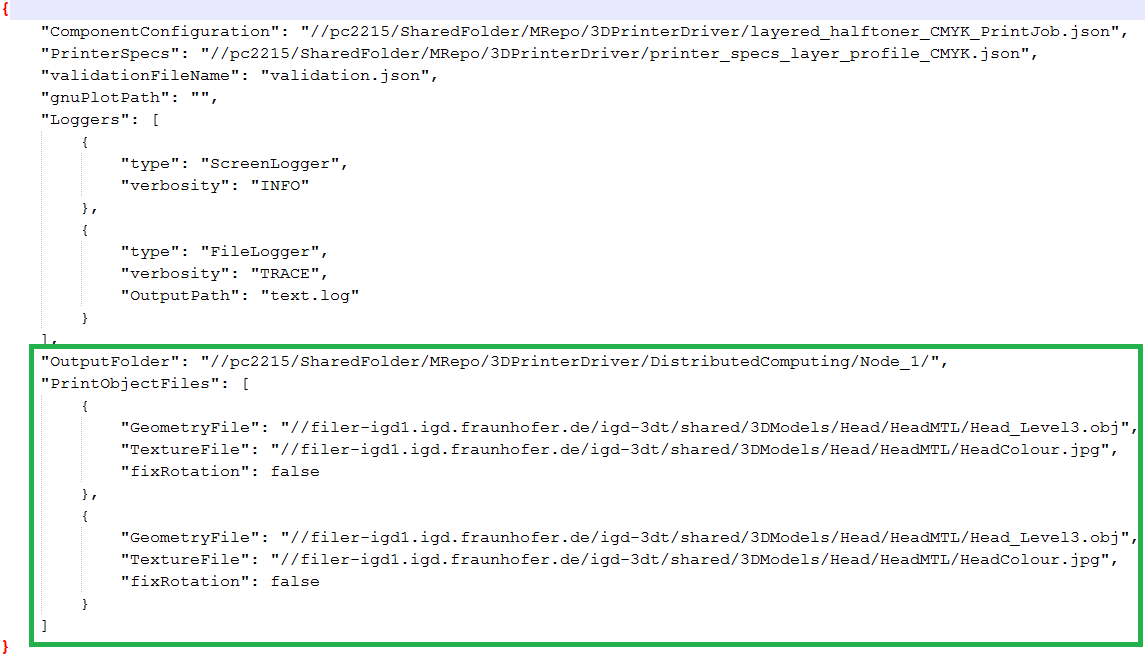
\includegraphics[scale=0.75]{Slave1ConfigurationFile.png}
\caption{Slave 1 Configuration file}
\label{fig:Slave1ConfigurationFile}
\end{figure}

\begin{figure}[ht!]
\centering
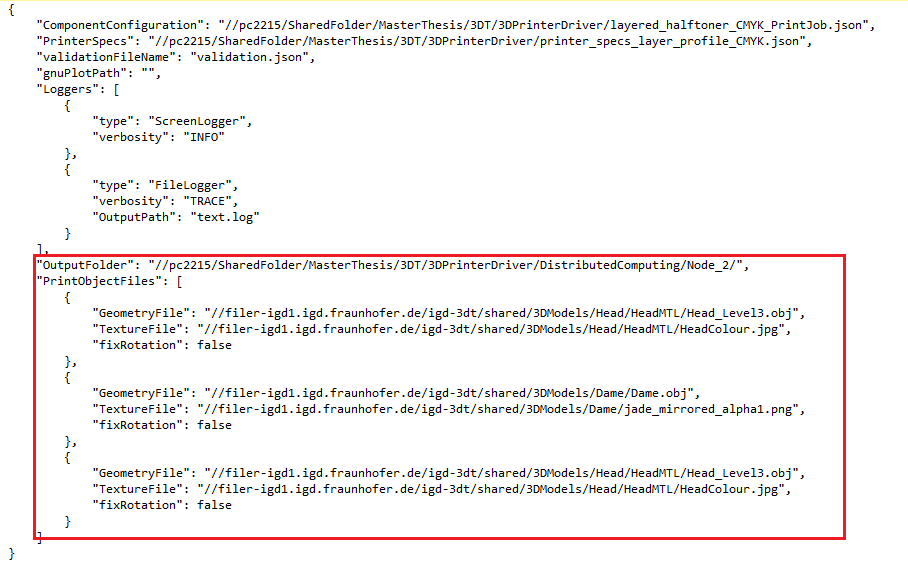
\includegraphics[scale=0.75]{Slave2ConfigurationFile.png}
\caption{Slave 2 Configuration file}
\label{fig:Slave2ConfigurationFile}
\end{figure}

This prototype is possible only if the cluster nodes have read/write permission to the shared network file system where the geometry,texture files and input/output folders are stored /created. The \textit{MasterDistributor} creates a unique path for each slave using the rank of the slave and writes the configuration file to this path. It then communicates to the slave only the path where the slave can find the configuration file. The sequence diagram in the figure \ref{fig:SequenceDiagram1} summarizes the communication between the master and the slaves.  

\begin{figure}[ht!]
\centering
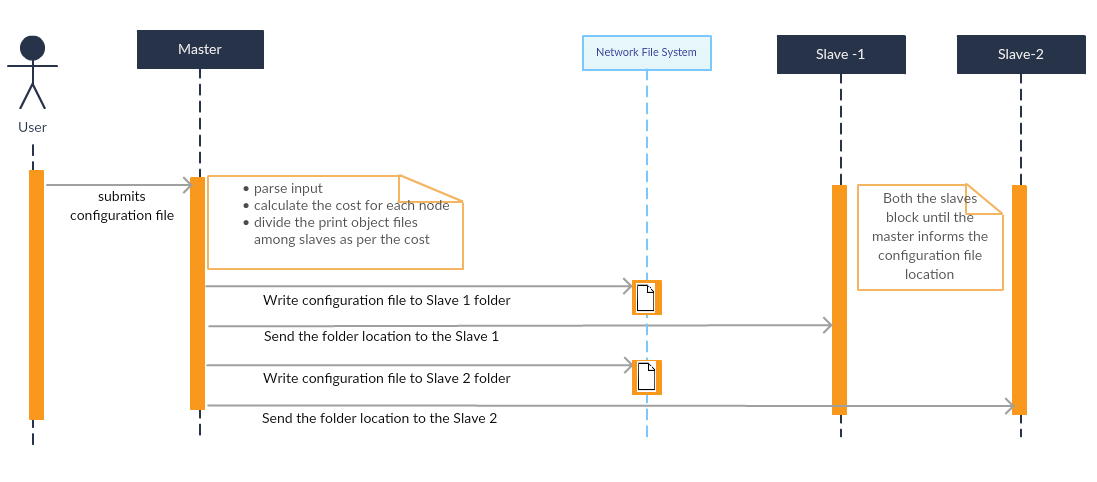
\includegraphics[scale=0.6]{SequenceDiagram1.png}
\caption{Master-slave input communication}
\label{fig:SequenceDiagram1}
\end{figure}

The pros of distributing the sub-tasks through the configuration file are:
\begin{itemize}
\item \textbf{Design simplicity}: The most important aspect of this design is it's simplicity as the \textit{SlavePrintingSoftware} pipeline does not need to be modified greatly which means that it is almost similar to running a single instance of the non-distributed version of the 3D Printing pipeline. 
\item \textbf{Lower Communication Overhead}: Slave nodes are blocked until the master communicates the configuration file path to each slave. Communication of the file path is faster as it very less number of bytes to be exchanged among the nodes as compared to the number of bytes to be sent when print jobs are distributed .
\item \textbf{Faster Disk I/O}: The configuration file read and writes i.e. disk I/O (both at the master and slave) are much faster than sending the print job as series of bytes. It is almost simpler implementation as communicating the print jobs as series of bytes would require defining a protocol for packing and unpacking of the print jobs with an additional effort at both master and slave nodes.
\item \textbf{No serialization and deserialization}: As the configuration files are in JSON format, there are very efficient library functions which allow to read and write the files with ease. As the format of the files is very standard, there is no need for serialization and deserialization of the files even if the nodes have varying underlying system architecture.        
\end{itemize}

The cons of distributing the sub-tasks via configuration file are: 
\begin{itemize}
\item \textbf{Dependency on shared network file system}: This prototype has a strong requirement that the nodes have a shared network file system and each node must have read access to the model texture/geometry file along with write access to the output folder to dump the partial output. If the print jobs are communicated as stream of bytes, it is possible to get rid of this requirement.
\item \textbf{Performance overhead}: The configuration file , model geometry and texture files are parsed twice, once by the master to create the prints jobs needed for cost computation and once by the slaves for actual computation. This leads to redundant execution of the \textit{FileParserPj} and \textit{PrintJobOrganizer} at both master and slave nodes which accumulates to a significant performance overhead.
\item \textbf{Disk I/O performance limited by network bandwidth}: As the files are read and written to the shared network file system, the network bandwidth limits the speed of the disk I/O. With increase in number of slave nodes, the load at the master to write the configuration file per slave increases which may become a performance bottleneck. 
\end{itemize}

\subsection{Slave Partial Output}


\subsection{Partial Output Merging at Master} 

\section{Prototype II- Input/Output independent of NFS }

\begin{figure}
\centering
\begin{tikzpicture}[node distance=2.75cm] 
\node (start) [startstop] {Start};
\node (dec1) [decision,below of=start ,yshift=-0.75cm]{ Is master node?};
\node (Min1) [io, below left of=dec1 , xshift= -2cm] {Input main configuration file};
\node (Sin1) [io,below right of=dec1 , xshift= 2cm] {Receive sub-tasks from Master};
\node (Mpro1) [process, below of=Min1] {Parse Input, Create sub-tasks, Distribute Sub-tasks};
\node (Mpro2) [process, below of=Mpro1 ,yshift=-0.5cm] {Receive meta-data, compute full slice height, width, offset};
\node (Mpro3) [process, below of=Mpro2 ,yshift=-0.5cm] {Receive partial slices and merge to full slice};
\node (Mdec1) [decision,below of=Mpro3, yshift=-0.5cm]{ Is last slice?};
\node (Spro1) [process, below of=Sin1] {Perform computation and generate chunk-wise slices };
\node (Sdec1) [decision,below of=Spro1, yshift=-0.5cm]{ Is first chunk?};
\node (Spro2) [process, below left of=Sdec1,xshift= -1cm] {Send meta-data to the master};
\node (Spro3) [process, below of=Sdec1,yshift=-1cm ] {Send the partial slice to the master};
\node (Sdec2) [decision,below of=Spro3, yshift=-0.5cm]{ Is last chunk?};
\node (Mend) [startstop,below of= Mdec1 , yshift=-1.5cm] {End};
\node (Send) [startstop,below of=Sdec2, yshift=-1.25cm ] {End};

\draw [arrow] (start) -- (dec1);
\draw [arrow] (dec1) -| node {yes}(Min1);
\draw [arrow] (dec1) -| node {no}(Sin1);
\draw [arrow] (Min1) -- (Mpro1);
\draw [arrow] (Mpro1) -- (Mpro2);
\draw [arrow] (Mpro2) -- (Mpro3);
\draw [arrow] (Mpro3) -- (Mdec1);
\draw [arrow] (Mdec1.west) -|node {no} ++(-0.5,0)|-(Mpro3.west);
\draw [arrow] (Mdec1) -- node {yes}(Mend);
\draw [arrow] (Sin1) -- (Spro1);
\draw [arrow] (Spro1) -- (Sdec1);
\draw [arrow] (Sdec1) -| node {yes}(Spro2);
\draw [arrow] (Sdec1) -- node {no}(Spro3);
\draw [arrow] (Spro2) -| (Spro3);
\draw [arrow] (Spro3) -- (Sdec2);
\draw [arrow] (Sdec2.east)-|node {no} ++(0.5,0)|-(Spro1.east);
\draw [arrow] (Sdec2) -- node {yes}(Send);
\end{tikzpicture}
\caption{Distributed Printer Driver Flow Chart}
\label{lst:FC}
\end{figure}




